\documentclass[xetex,dvipsnames]{beamer}

\usepackage{fontspec}                           	% Typo
\usepackage[french,english]{babel}
\usepackage{empheq}                             	% Encadrer les équations
\usepackage{amsthm}                             	% Démonstration de maths
\usepackage{tabularx}                           	% Tableaux avancés
\usepackage{fancyvrb}                           	% Blocs mono avancés
\usepackage{caption}                            	% Légendes avancées
\usepackage{tikz}                               	% Outil de dessin
\usepackage{listings}                           	% Coloration syntaxique
\usepackage{xcolor}                             	% Color support
\usepackage{enumerate}
\usetikzlibrary{calc,arrows,shapes.misc}
\usepackage{hyperref}

\tikzset{cross/.style={cross out, draw=black, minimum size=8*(#1-\pgflinewidth), inner sep=0pt, outer sep=0pt},cross/.default={1pt}}
\definecolor{salmon}{HTML}{FA8072}
\usefonttheme[onlymath]{serif} % Force les maths en serif

%%%%%%%%%%%%%%%%%%%%%
\usetheme{Frankfurt}	
\usecolortheme[rgb={0,0.6,0}]{structure}
\captionsetup{font=scriptsize,labelfont=scriptsize}
\setbeamertemplate{caption}{\raggedright\insertcaption\par}
%%%%%%%%%%%%%%%%%%%%%

\begin{document}


% Agmente les marges entre paragraphes % \setlength{\parskip}{1em}
\title{Introduction aux Bases de Données}

% Numerotations
\addtobeamertemplate{navigation symbols}{} { \usebeamerfont{footline} \usebeamercolor[fg]{footline} \hspace{1em} \insertframenumber/\inserttotalframenumber }


\author{Ulysse COUTAUD\\\href{mailto:ulysse.coutaud@gmail.com}{\small ulysse.coutaud@gmail.com}}
\date{}
	
\maketitle

\section{Introduction}

\begin{frame}{Base de données (BDD) ?}
    \begin{columns}
	    \begin{column}{0.5\textwidth}
	    Ensemble d'informations:
		 	\begin{itemize}
		 		\item Stockées.
		 		\item Consultées.
		 		\item Modifiées.
		 	\end{itemize}
		\end{column}
		\begin{column}{0.5\textwidth}
\begin{footnotesize}
		Exemples:
			\begin{itemize}
		 		\item Carnet d'adresses (quelques kilobytes).
		 		\item Comptes bancaires.
		 		\item Registre des personnels, des accès.
		 		\item Réservations des places dans les trains.
		 		\item Suivi des stocks, de la production, des commandes.
		 		\item Données de supervisions, programmes d'usinages, ...
		 		\item World Data Centre for Climate (6 petabytes).
		 	\end{itemize}
\end{footnotesize}
		\end{column}
	\end{columns}
		
\end{frame}

\begin{frame}[t]{Système de Gestion de Base de Données (SGBD) ?}
	     \begin{exampleblock}{}
	     	Ensemble d'outils permettant \textbf{l'organisation, le contrôle, la consultation et la modification} d'une base de donnée.
	     \end{exampleblock}
  \begin{columns}
	    \begin{column}{0.6\textwidth}
\begin{footnotesize}
	  	\begin{itemize}
	  		\item Accès et manipulation standardisés.
		 	\begin{itemize}
		 	\item Indépendance physique des données
	  		\item Indépendance logique des données
	  		\item Réduire la complexité
	 		\item Stockage et accès optimisés.
		 	\end{itemize}
		 	\item Contrôle de cohérence des données
		 	\item Sécurité des données
		 	\item Accès ou transactions (massivement) concurrentes.
		 	\item Fiabilité (sauvegardes, restaurations, ...)
		 	\end{itemize}
\end{footnotesize}
		\end{column}
		\begin{column}{0.4\textwidth}
		\begin{figure} \begin{center}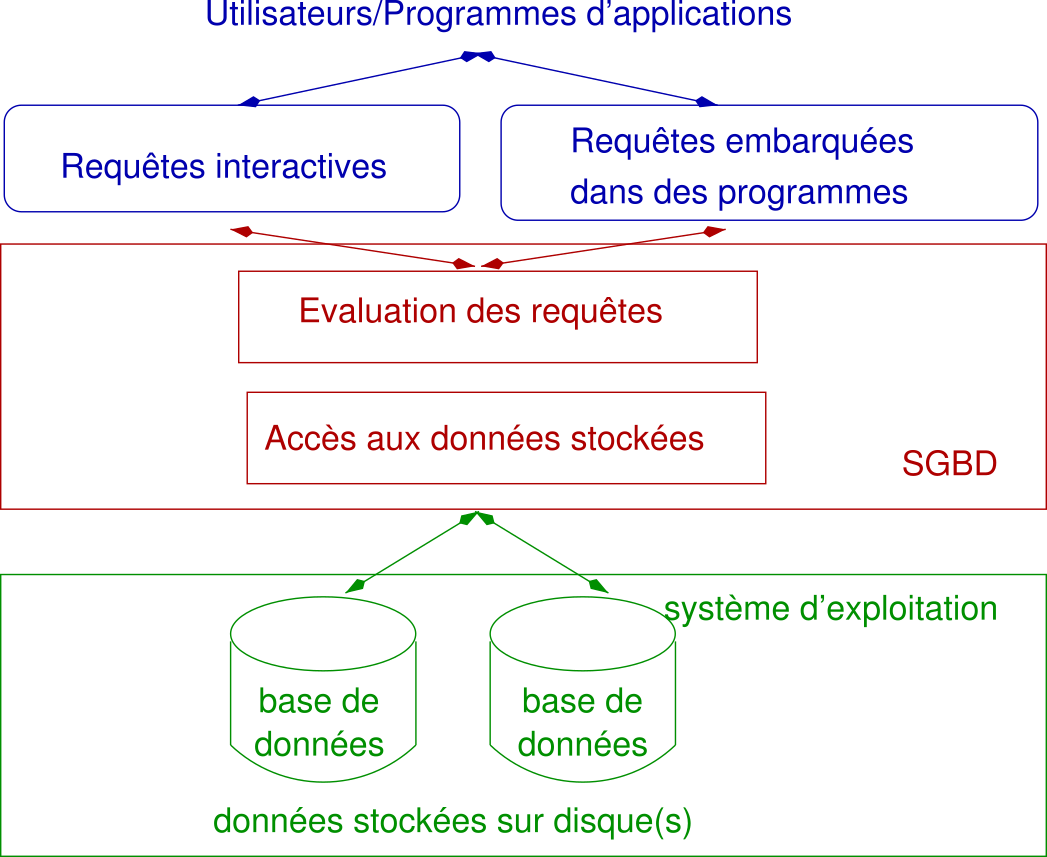
\includegraphics[width=0.99\textwidth]{./figures/SGBDR.png}\end{center}\end{figure}
		\end{column}
	\end{columns}
\end{frame}

\begin{frame}{Un exemple}
Un outil de gestion d'atelier: GEDIX.
\end{frame}

\begin{frame}{Dans ce cours}
Rudiments des Bases de Données:
\begin{itemize}
	\item Le modèle "relationnel"
	\item Le langage SQL
	\item PostgreSQL
	\item Lire les données
	\item Modifier les données
	\item Concevoir une base de données simple
\end{itemize}
\end{frame}



\begin{frame}{Un peu de vocabulaire}
	\begin{itemize}
		\item \textbf{BDD} Base De Données
		\item \textbf{DB} Database
	\end{itemize}
	\vspace{1em}
	\begin{itemize}
		\item \textbf{SGBD} Système de Gestion de Base de Données 
		\item \textbf{DBMS} Data Base Management System
	\end{itemize}
	\vspace{1em}
	\begin{itemize}
			\item \textbf{SGBDR} Système de Gestion de Base de Données Relationnelles
			\item \textbf{RDBMS} Relational Database Management System 
	\end{itemize}
	\vspace{1em}
%	\begin{itemize}
%		\item \textbf{DBA} Database Administrator
%	\end{itemize}
	
	\begin{itemize}
		\item \textbf{SQL} Structured Query Language : Norme/langage de manipulation de données relationnelles.
	\end{itemize}
\end{frame}

\begin{frame}{Les principaux acteurs}
    \begin{columns}
    \begin{column}{0.6\textwidth}
	\begin{itemize}
		\item 
\includegraphics[width=0.3\textwidth]{./figures/oracle.png} :
		\begin{itemize}
			\item Oracle DB 
			\item 
\includegraphics[width=0.14\textwidth]{./figures/mysql.png}
		\end{itemize}
		\item Microsoft
		\begin{itemize} 
			\item MS SQL: 
\includegraphics[width=0.12\textwidth]{./figures/mssql.png}
			\item Microsoft Access:  
\includegraphics[width=0.07\textwidth]{./figures/access.png}
		\end{itemize}
		\item IBM: IBM DB2 
\includegraphics[width=0.09\textwidth]{./figures/IBMDB2.png}
		\item SQLlite: 
\includegraphics[width=0.12\textwidth]{./figures/sqllite.png}
	\end{itemize}
	    \end{column}
		\begin{column}{0.5\textwidth}
		\begin{center}
	    	
\includegraphics[width=0.4\textwidth]{./figures/postgressql.png}
	    \end{center}
		\begin{itemize}
			\item \textbf{PostgreSQL}
			\item Open source
			\item Université de Berkeley
			\item Très populaire et répandu \footnote{{\tiny \url{https://db-engines.com/en/ranking_trend/relational+dbms}}}
		\end{itemize} 
	    \end{column}

    \end{columns}
\end{frame}



\section{Le modèle relationnel}
\begin{frame}{Le modèle relationnel}
		\begin{center}
			Une TABLE = une "RELATION"
	    \end{center}
			\vspace{0.3em}
	    	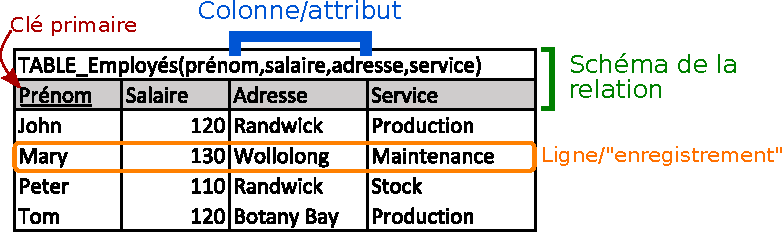
\includegraphics[width=0.8\textwidth]{./figures/relation.pdf}
	    	\vspace{0.3em}
	    	\pause
	    	\vspace*{0.3em}
\begin{flushright}
	    	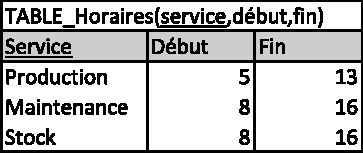
\includegraphics[width=0.55\textwidth]{./figures/relation2.pdf}
\end{flushright}
 			\begin{center}
			L'ensemble des schémas de relations + liens entre eux = le schéma de la base de données.
	    \end{center}
\end{frame}


\section{Consulter des données en SQL}
\begin{frame}{Se connecter à la base de données}
 	\begin{center}
	    	\begin{figure}
	    	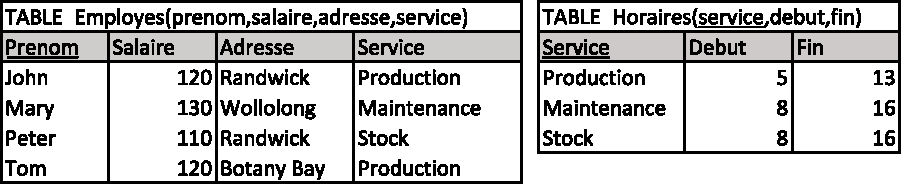
\includegraphics[width=0.85\textwidth]{./figures/BDDatelier.pdf}
	    	\caption{BDD "atelier"}
	    	\end{figure}
	\end{center}
	\begin{itemize}
		\item Ouvrir ligne de commande (Win + cmd)
		\item Taper "psql fabrique postgres"
		\item Entrer le mot de passe "postgres"
		\item Lister les tables de la BDD courante \textbackslash dt
	\end{itemize}		
\end{frame}

\begin{frame}{Clause SELECT}
	BDD "atelier":
 	\begin{center}
	    	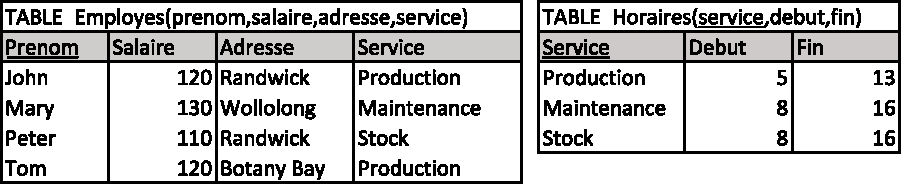
\includegraphics[width=0.85\textwidth]{./figures/BDDatelier.pdf}
	\end{center}
	\begin{alertblock}{Afficher toute la table}
		SELECT * FROM nom\_table;
	\end{alertblock}
	\begin{alertblock}{Afficher certaines colonnes}
		SELECT colonne1, colonne2 FROM table;
	\end{alertblock}
		\textit{Afficher les prénoms et salaires des employés.}\\
		\textit{Afficher toutes les informations des employés.}
\end{frame}

\begin{frame}[t]{Clause SELECT avec contraintes}
\begin{small}
		BDD "atelier": \\employes(\underline{prenom},salaire,adresse,service) horaires(\underline{service},debut,fin)
\end{small}	\begin{alertblock}{}
		SELECT colonne1, colonne2 FROM tableau WHERE condition1 AND/OR NOT condition2;
	\end{alertblock}
	
\begin{footnotesize}
 \begin{columns}
    \begin{column}{0.5\textwidth}
	\begin{block}{Nombres:}
		=, !=, <, <=, >, >=,
		\\BETWEEN nombre1 AND nombre2,
		\\IN (nombre1, nombre2, nombre3)
	\end{block}
	    \end{column}
	    \begin{column}{0.5\textwidth}
		\begin{block}{Texte:}
Sensible à la casse: =, != ou <> 
\\Non sensible à la casse: LIKE (caractère joker: \%)
\\IN ("mot1", "mot2", "mot3")
	\end{block}
		    \end{column}
	    \end{columns}

\end{footnotesize}
		\textit{Afficher les prénoms des employés du service production.}\\
		\textit{Afficher les prénoms des employés qui gagne 110 ou moins.}\\
		\textit{Afficher les prénoms des employés dont l'adresse contient la chaine "an".}\\
		\textit{Afficher les prénoms et salaires des employés du service Production et Maintenance.}\\
\end{frame}


\begin{frame}[t]{Filtrer les résultats}
\begin{small}
		BDD "atelier": \\employes(\underline{prenom},salaire,adresse,service) horaires(\underline{service},debut,fin)
\end{small}	
	\begin{alertblock}{Clause DISTINCT}
		SELECT DISTINCT colonne1 FROM table;
	\end{alertblock}
	
		\textit{Afficher sans répétition la liste des services.}\\
		\textit{Afficher sans répétition les débuts de services.}\\
\end{frame}


\begin{frame}[t]{Filtrer les résultats}
\begin{small}
		BDD "atelier": \\employes(\underline{prenom},salaire,adresse,service) horaires(\underline{service},debut,fin)
\end{small}	
	\begin{alertblock}{Clause ORDER BY}
		SELECT colonne1 FROM table ORDER BY colonne1 ASC/DESC;
	\end{alertblock}
	
		\textit{Afficher toutes les informations sur les employes en les triants par ordre alphabétique sur les prénoms.}\\
		\textit{Afficher prénoms et adresses des employes en triant par salaires décroissants.}\\
\end{frame}


\begin{frame}[t]{Filtrer les résultats}
\begin{small}
		BDD "atelier": \\employes(\underline{prenom},salaire,adresse,service) horaires(\underline{service},debut,fin)
\end{small}	
	\begin{alertblock}{Clauses LIMIT et OFFSET}
		SELECT colonne1 FROM table LIMIT num\_limit OFFSET num\_offset;
	\end{alertblock}
		\textit{Afficher l'employé le moins bien payé.}\\
		\textit{Afficher le deuxieme employé le moins bien payé.}\\
\end{frame}

\begin{frame}[t]{Requêtes sur plusieurs tables}
\begin{small}
		BDD "atelier": \\employes(\underline{prenom},salaire,adresse,service) horaires(\underline{service},debut,fin)
\end{small}	
	\begin{alertblock}{Clause INNER JOIN}
		SELECT colonne1 FROM table1 INNER JOIN table2 ON table1.colonneX=table2.colonneY;
	\end{alertblock}
\begin{footnotesize}
	\begin{block}{Remarque}
	 1: Le INNER JOIN est le JOIN par defaut, le mot clé "INNER" n'est pas nécessaire.
	\\2: En cas d'ambiguité sur le nom de colonne, on ajoute en préfixe la table visé (ex: table1.colonne1). On peut également renommer la colonne résultat avec le mot clé "AS" (ex: table1.colonne1 AS T1C1)
	\end{block}
\end{footnotesize}
		
		\textit{Afficher la jonction de toutes les informations de la BDD}\\
		\textit{Afficher les horaires de John.}\\
		\textit{Afficher les noms et horaires de tous les employés du service production.}\\
\end{frame}

\begin{frame}[t]{Requêtes sur plusieurs tables}
\begin{small}
		BDD "atelier": \\employes(\underline{prenom},salaire,adresse,service) horaires(\underline{service},debut,fin)
\end{small}	
	\begin{alertblock}{LEFT JOIN}
		Il y aura forcément chacune des lignes de table1. Si aucune correspondance avec table2: NULL.
	\end{alertblock}
	\begin{alertblock}{RIGHT JOIN}
		Il y aura forcément chacune des lignes de table2. Si aucune correspondance avec table1: NULL.
	\end{alertblock}
\begin{footnotesize}
	\begin{block}{Valeur NULL}
		Se filtre avec IS NULL ou IS NOT NULL
	\end{block}
\end{footnotesize}
		
		\textit{Afficher les prénoms des employés qui n'ont pas d'horaires.}\\

\end{frame}

\begin{frame}[t]{Les expressions}
\begin{small}
		BDD "atelier": \\employes(\underline{prenom},salaire,adresse,service) horaires(\underline{service},debut,fin)
\end{small}	
	\begin{alertblock}{}
	SELECT colonne1, colonne2  * 10 AS colonne2\_pourcent FROM table;\\
	SELECT colonne1, colonne2 FROM table WHERE colonne2 * 10 > 80;
	\end{alertblock}

	\textit{Les salaires de la base sont journaliers. Afficher les prénoms et salaires mensuels (20 jours travaillés).}
\end{frame}

\begin{frame}[t]{Les aggrégats}
\begin{small}
		BDD "atelier": \\employes(\underline{prenom},salaire,adresse,service) horaires(\underline{service},debut,fin)
\end{small}	
	\begin{alertblock}{}
	SELECT COUNT(colonne1) from table;
	\end{alertblock}
	\begin{block}{Les fonctions d'aggrégats:}
		COUNT, MIN, MAX, AVG, SUM.	
	\end{block}

	\textit{Afficher le nombre d'employés.}\\
	\textit{Afficher le salaire minimal.}\\
	\textit{Afficher le salaire moyen.}\\
	\textit{Afficher la masse salariale totale.}\\

\end{frame}

\begin{frame}[t]{Les aggrégats}
\begin{small}
		BDD "atelier": \\employes(\underline{prenom},salaire,adresse,service) horaires(\underline{service},debut,fin)
\end{small}	
	\begin{alertblock}{Clause GROUP BY}
	SELECT colonne1, SUM(colonne2) FROM table GROUP BY colonne1;
	Applique la fonction d'aggrégat à chaque groupe ayant la même valeur en colonne1.
	\end{alertblock}
	\textit{Afficher la masse salariale de chaque service.}\\
	\textit{Afficher le salaire moyen par adresse.}\\
	
	\begin{alertblock}{Clause HAVING}
	Equivalent de WHERE pour les expressions.
	\end{alertblock}
	\textit{Afficher le salaire moyen des groupes d'employés ayant tous le même salaire à une même adresse.}\\
\end{frame}



\end{document}
